\documentclass[]{standalone}
\usepackage{tikz}


\begin{document}
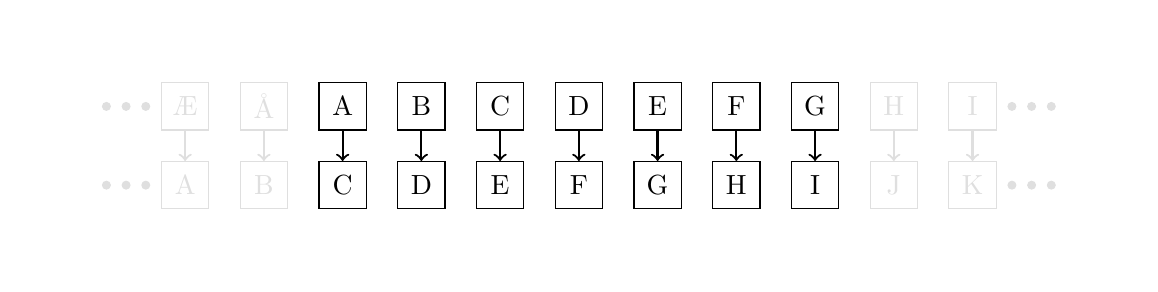
\begin{tikzpicture}
\node[draw, minimum height= .6cm, minimum width= .6cm](A) at (0,0) {A};
\node[draw, minimum height= .6cm, minimum width= .6cm](B) at (1,0) {B};
\node[draw, minimum height= .6cm, minimum width= .6cm](C) at (2,0) {C};
\node[draw, minimum height= .6cm, minimum width= .6cm](D) at (3,0) {D};
\node[draw, minimum height= .6cm, minimum width= .6cm](E) at (4,0) {E};
\node[draw, minimum height= .6cm, minimum width= .6cm](F) at (5,0) {F};
\node[draw, minimum height= .6cm, minimum width= .6cm](G) at (6,0) {G};


\node[draw, minimum height= .6cm, minimum width= .6cm](c) at (0,-1) {C};
\node[draw, minimum height= .6cm, minimum width= .6cm](d) at (1,-1) {D};
\node[draw, minimum height= .6cm, minimum width= .6cm](e) at (2,-1) {E};
\node[draw, minimum height= .6cm, minimum width= .6cm](f) at (3,-1) {F};
\node[draw, minimum height= .6cm, minimum width= .6cm](g) at (4,-1) {G};
\node[draw, minimum height= .6cm, minimum width= .6cm](h) at (5,-1) {H};
\node[draw, minimum height= .6cm, minimum width= .6cm](i) at (6,-1) {I};

\node[draw, gray!25, minimum height= .6cm, minimum width= .6cm](AE) at (-2, 0) {Æ};
\node[draw, gray!25, minimum height= .6cm, minimum width= .6cm](AA) at (-1, 0) {Å};
\node[draw, gray!25, minimum height= .6cm, minimum width= .6cm](a) at (-2, -1) {A};
\node[draw, gray!25, minimum height= .6cm, minimum width= .6cm](b) at (-1, -1) {B};


\node[draw, gray!25, minimum height= .6cm, minimum width= .6cm](H) at (7, 0) {H};
\node[draw, gray!25, minimum height= .6cm, minimum width= .6cm](I) at (8, 0) {I};
\node[draw, gray!25, minimum height= .6cm, minimum width= .6cm](j) at (7, -1) {J};
\node[draw, gray!25, minimum height= .6cm, minimum width= .6cm](k) at (8, -1) {K};

\draw[thick, ->] (A) -- (c);
\draw[thick, ->] (B) -- (d);
\draw[thick, ->] (C) -- (e);
\draw[thick, ->] (D) -- (f);
\draw[thick, ->] (E) -- (g);
\draw[thick, ->] (F) -- (h);
\draw[thick, ->] (G) -- (i);


\draw[thick, ->, gray!25] (AE) -- (a);
\draw[thick, ->, gray!25] (AA) -- (b);
\draw[thick, ->, gray!25] (H) -- (j);
\draw[thick, ->, gray!25] (I) -- (k);

\node[draw, gray!25, circle, inner sep = 1pt, fill = gray!25] at (8.5, 0) {};
\node[draw, gray!25, circle, inner sep = 1pt, fill = gray!25] at (8.75, 0) {};
\node[draw, gray!25, circle, inner sep = 1pt, fill = gray!25] at (9, 0) {};

\node[draw, gray!25, circle, inner sep = 1pt, fill = gray!25] at (8.5, -1) {};
\node[draw, gray!25, circle, inner sep = 1pt, fill = gray!25] at (8.75, -1) {};
\node[draw, gray!25, circle, inner sep = 1pt, fill = gray!25] at (9, -1) {};



\node[draw, gray!25, circle, inner sep = 1pt, fill = gray!25] at (-2.5, 0) {};
\node[draw, gray!25, circle, inner sep = 1pt, fill = gray!25] at (-2.75, 0) {};
\node[draw, gray!25, circle, inner sep = 1pt, fill = gray!25] at (-3, 0) {};

\node[draw, gray!25, circle, inner sep = 1pt, fill = gray!25] at (-2.5, -1) {};
\node[draw, gray!25, circle, inner sep = 1pt, fill = gray!25] at (-2.75, -1) {};
\node[draw, gray!25, circle, inner sep = 1pt, fill = gray!25] at (-3, -1) {};
\path (-4, -2) -- (10,1);
\end{tikzpicture}
\end{document}
